%
% Documento: Fundamentação Teórica
%

\chapter{Fundamentação Teórica}
\label{chap:fundamentacaoTeorica}

Neste capítulo, são abordados os temas necessários para a compreensão do trabalho desenvolvido. Na Seção \ref{sec:fundamentacaoTeorica-sistemas-controle} é apresentada uma introdução aos sistemas de controle, na \ref{sec:fundamentacaoTeorica-rna}, é discutido o que é uma Rede Neural Artificial (RNA), na \ref{sec:fundamentacaoTeorica-fuzzy} se trata da lógica fuzzy e, por fim, na Seção \ref{sec:fundamentacaoTeorica-neuro-fuzzy} é apresentada a rede neuro-fuzzy.

\section{Sistemas de Controle}
\label{sec:fundamentacaoTeorica-sistemas-controle}

%Professor, a seção de Sistemas de Controle ainda não finalizada e, portanto, seu conteúdo não é exibido aqui.
Um sistema de controle é, segundo \citeonline[p.~2]{Dorf2011}, uma interconexão de componentes formando uma configuração de sistema que vai fornecer uma resposta desejada. Todo sistema de controle tem, como objetivo, atuar sobre um determinado processo, o qual pode ser representado por um bloco que representa a relação entre entrada e saída do sistema, como mostrado na Figura \ref{fig:process}.

\begin{figure}[!htb]
    \centering
    \caption{Diagrama representando um processo}
    
\includegraphics[width=0.7\textwidth]{./04-figuras/fund_teorica/process}
    \fonte{Adaptado de \citeonline[p.~2]{Dorf2011}}
    \label{fig:process}
\end{figure}

O controle de um processo pode assumir duas formas distintas: malha aberta ou malha fechada, sendo que um sistema de controle em malha aberta é composto, além do processo, por um controlador e um atuador para se obter a resposta desejada sem o uso de realimentação \cite[p.~2]{Dorf2011}. Um exemplo de sistema deste tipo é mostrado na Figura \ref{fig:open_loop_control_system}.

\begin{figure}[!htb]
    \centering
    \caption{Diagrama representando um sistema de controle em malha aberta}
    
\includegraphics[width=0.95\textwidth]{./04-figuras/fund_teorica/open_loop_control_system}
    \fonte{Adaptado de \citeonline[p.~2]{Dorf2011}}
    \label{fig:open_loop_control_system}
\end{figure}

Em oposição a um sistema de controle em malha aberta, um em malha fechada incorpora, além dos componentes que aquele inclui, uma medição dos estados atuais para serem comparados com os valores desejados para o processo. Um exemplo de um sistema de controle em malha fechada simples é mostrado na Figura \ref{fig:closed_loop_control_system}. Os sistemas em malha fechada apresentam várias vantagens sobre os em malha aberta como, por exemplo, a capacidade de rejeitar distúrbios externos e melhorar a atenuação de ruídos nas medições, elementos estes que são inevitáveis em aplicações no mundo real \cite[p.~3]{Dorf2011}.

\begin{figure}[!htb]
    \centering
    \caption{Diagrama representando um sistema de controle em malha fechada}
    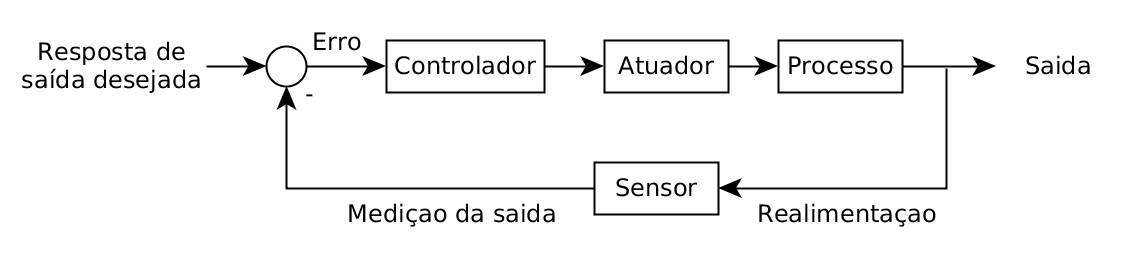
\includegraphics[width=0.95\textwidth]{./04-figuras/fund_teorica/closed_loop_control_system}
    \fonte{Adaptado de \citeonline[p.~3]{Dorf2011}}
    \label{fig:closed_loop_control_system}
\end{figure}

Como já foi visto, um processo representa a relação entre a entrada e a saída de um sistema sendo que há diferentes formas de fazê-lo. Uma forma de representar sistemas contínuos e é utilizando o espaço de estados.

%\subsection{Funções de Transferência}
%\label{subsec:fundamentacaoTeorica-tfs}
%%Ogata 15 do pdf; Dorf 65 do pdf
A função de transferência de um sistema representa a relação que descreve as dinâmicas do sistema em questão e é definida pela razão entre as transformadas de Laplace das variáveis de saída e de entrada com todas as condições iniciadas definidas como zero \cite[p.~65]{Dorf2011}. A forma de uma função de transferência é dada a seguir:
\begin{center}
$G(s) = \frac{Y(s)}{X(s)}$
\end{center}
em que $G(s)$ é a função de transferência que descreve o sistema, $Y(s)$ é a transformada de Laplace da variável de saída do sistema e $X(s)$ é a transformada de Laplace da variável de entrada, ambas considerando as condições iniciais definidas como zero.

Apesar de ser amplamente utilizada, o uso de funções de transferência tem certas limitações. As transformadas de Laplace só podem ser utilizadas sobre sistemas descritos por equações e diferencias lineares e sem parâmetros variantes no tempo e, portanto, o uso das funções de transferência se restringem aos casos em que estas condições são satisfeitas.

Além da representação a partir de funções de transferência, uma forma alternativa de representar as dinâmicas do sistema é a representação no espaço de estados.



\subsection{Espaço de Estados}
\label{subsec:fundamentacaoTeorica-ss}

%Ogata 29 do pdf (digrma de blocos na pag 32); Dorf 165 do pdf
A representação de um sistema dinâmico no espaço de estados descreve um sistema a partir das seguintes equações :
\begin{center}\label{eq:k1}
%$\dot{x}(t)=A(t)x(t)+B(t)u(t)$ \\
%$y(t)=C(t)x(t)+D(t)u(t)$
$\dot{x}=Ax+Bu$ \\
$y=Cx+Du$
\end{center}
%em que $A(t)$ é a matriz de estados, $B(t)$ a matriz de entrada, $C(t)$ a matriz de saída, $D(t)$ a matriz de transmissão direta, $x$ é o vetor de variáveis de estado, $u$ o vetor de entradas e $y$ o vetor de saídas. A Figura \ref{fig:ss_diagram} exibe um diagrama de blocos para a representação em espaço de estados definida.
em que $A$ é a matriz de estados, $B$ a matriz de entrada, $C$ a matriz de saída, $D$ a matriz de transmissão direta, $x$ é o vetor de variáveis de estado, $u$ o vetor de entradas e $y$ o vetor de saídas. A Figura \ref{fig:ss_diagram} exibe um diagrama de blocos para a representação em espaço de estados definida.

\begin{figure}[!htb]
    \centering
    \caption{Diagrama de blocos de um sistema linear e contínuo tempo representado no espaço de estados}
    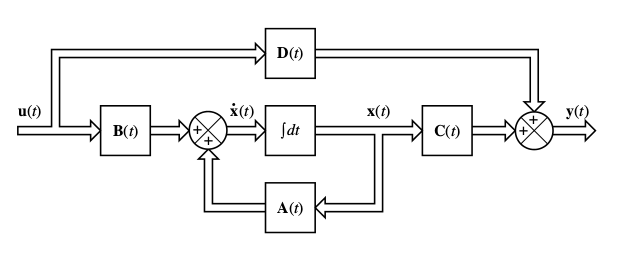
\includegraphics[width=0.9\textwidth]{./04-figuras/fund_teorica/ss_diagram}
    \fonte{\citeonline[p.~32]{Ogata2010}}
    \label{fig:ss_diagram}
\end{figure}

A representação no espaço de estados oferece uma ferramenta poderosa para a manipulação da representação do sistema, permitindo que as variáveis de estado sejam representadas de forma independente entre si a partir do processo de desacoplamento delas.

O processo de desacoplamento de variáveis de estado é baseado em ferramentas matemáticas aplicando manipulações sobre frações parciais. A partir deste processo, por exemplo, o sistema mostrado na Figura \ref{fig:ss_coupled}, que representa um sistema de controle de um motor CC com velocidade como saída e é representado pela função de transferência:
\begin{equation}
G(s)=\frac{30(s+1)}{(s+5)(s+2)(s+3)}
\end{equation}
pode ser representado por uma função de transferência do tipo:
\begin{equation}
G(s)=\frac{q(s)}{(s-s_1)(s-s_2)(s-s_3)}
\end{equation}
cuja resposta é ditada por $s_1$, $s_2$ e $s_3$. Utilizando a expansão de frações parciais, pode-se representar a mesma função de transferência por \cite[p.~183]{Dorf2011}:
\begin{equation}
T(s)=\frac{k_1}{s+5}+\frac{k_2}{s+2}+\frac{k_3}{s+3}
\end{equation}

\begin{figure}[!htb]
    \centering
    \caption{Diagrama de blocos representando o controle de um motor CC com velocidade como saída}
    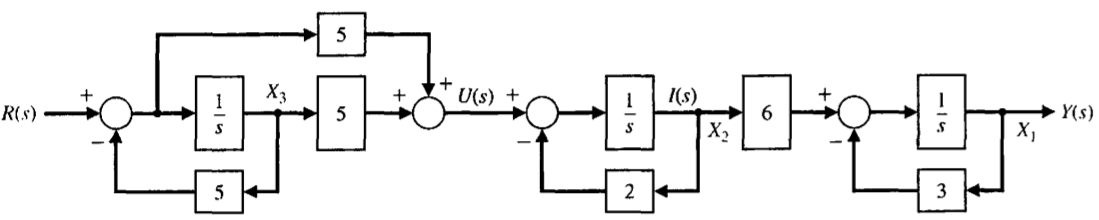
\includegraphics[width=1\textwidth]{./04-figuras/fund_teorica/ss_coupled_blocks}
    \fonte{\citeonline[p.~182]{Dorf2011}}
    \label{fig:ss_coupled}
\end{figure}

A partir de manipulações matemáticas relacionadas à expansão de frações parciais, constata-se que $k_1=-20$, $k_2=-10$ e $k_3=30$ \cite[p.~182]{Dorf2011}. Com isto, o sistema exibido na Figura \ref{fig:ss_coupled} pode ser representado como mostrado na Figura \ref{fig:ss_decoupled} que, como se pode ver, trata $X_1$, $X_2$ e $X_3$ de forma completamente independente e somando suas respectivas contribuições em $Y(s)$. Desta forma, pode-se ver claramente como cada variável de estado contribui para a saída ($Y(s)$) a partir de uma dada entrada ($X(s)$).

\begin{figure}[!htb]
    \centering
    \caption{Diagrama de blocos representando o controle de um motor CC com velocidade como saída e implementando desacoplamento das variáveis de estado}
    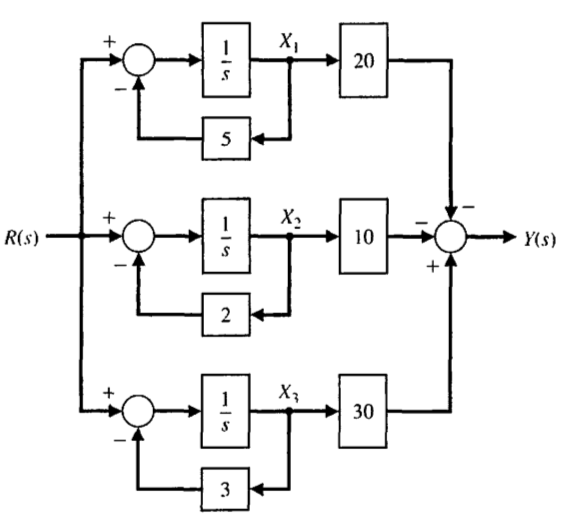
\includegraphics[width=0.6\textwidth]{./04-figuras/fund_teorica/ss_decoupled_blocks}
    \fonte{\citeonline[p.~182]{Dorf2011}}
    \label{fig:ss_decoupled}
\end{figure}










%No contexto deste trabalho, utilizou-se um sistema de controle em malha fechada no qual o processo a ser controlado diz respeito a um quadrotor. Além disto, os controladores utilizados foram de tipos bastante específicos: fuzzy e neuro-fuzzy, temas que são tratados nas próximas seções.

%Desacoplamento: Dorf pag 182 do pdf


\section{Redes Neurais Artificiais}
\label{sec:fundamentacaoTeorica-rna}
%redes neurais - pag 197 de jang
%adaptive networks - pag 199

%o que são redes neurais
Redes Neurais Artificiais (RNAs) são modelos computacionais bioinspirados no sistema neurológico humano. A motivação para o desenvolvimento e uso destes modelos é a grande complexidade do cérebro humano, definido por \citeonline{Haykin1998} como um computador altamente complexo, não linear e paralelo. O autor ainda define uma RNA como``\textit{a machine that is designed to} model \textit{the way in which the brain performs a particular task or function of interest}''\footnote{``uma máquina que é desenvolvida para \textit{modelar} a forma como o cérebro desempenha uma tarefa específica ou função de interesse'' (tradução nossa).}. Seguindo o modelo biológico do cérebro humano, uma RNA é composta por neurônios artificiais e pelas interações existentes entre estes neurônios: as sinapses.

%Explicação simplificada do sistema nervoso
A \autoref{fig:brainsistem} ilustra, em um diagrama de blocos, o sistema nervoso como um sistema de três estágios. A Rede Neural representa o cérebro em si, que recebe informações continuamente, as percebe e toma as decisões apropriadas para cada uma delas \cite[p.~24]{Haykin1998}.

\begin{figure}[!htb]
    \centering
    \caption{Representação em digrama de blocos do sistema nervoso}
    
\includegraphics[width=0.9\textwidth]{./04-figuras/brain_sistem_block_diagram}
    \fonte{Adaptado de \citeonline[p.~28]{Haykin1998}}
    \label{fig:brainsistem}
\end{figure}

%O que são sinapses
Toda esta comunicação se dá a partir de sinapses, que são unidades estruturais e funcionais que mediam a interação entre neurônios. Seu funcionamento simplificado é o seguinte: o processo pré-sináptico libera uma substância transmissora que é difundida através da junção sináptica entre neurônios e então age sobre o processo pós-sináptico. Então, a sinapse converte o sinal elétrico pré-sinápitico em um sinal químico e, por fim, de volta a um sinal elétrico pós-sináptico \cite[p.~28]{Haykin1998}. É por meio deste processo de comunicação entre neurônios que adquirimos novos conhecimentos e relacionamos estímulos a respostas. É também devido a ele que podemos fazer associações diversas com acontecimentos no passado, evento que chamamos de \textit{memória}. O imenso poder que os neurônios possuem inspirou modelagens computacionais capazes de atuar em situações em que se deseja obter respostas adequadas a diferentes estímulos, e em outras relacionadas à memória e aprendizado. Um modelo neural comumente aplicado na literatura em problemas relacionados às RNAs é o perceptron. 

Um perceptron é um modelo computacional de um neurônio não linear e é ilustrado na Figura \ref{fig:neuronmodel}, em que $y_k$ é a saída do sistema obtido após o processamento neural relacionado às entradas $x_i$, cada qual contribuindo com um peso $w_{ki}$ para a junção de soma representada pelo bloco $\sum$. O processamento neural envolve ainda a função de ativação $\phi$ que, de acordo com o valor obtido na junção de soma, define o valor da saída $y_k$. Se o valor $v_k$ for maior que um limiar pré-determinado, a saída do sistema é ativada e terá o valor 1, caso contrário assumirá o valor 0, simulando assim o processo de transmissão ou não de impulsos elétricos que ocorrem nos neurônios biológicos.

\begin{figure}[!htb]
    \centering
    \caption{Modelo não linear de um neurônio}
    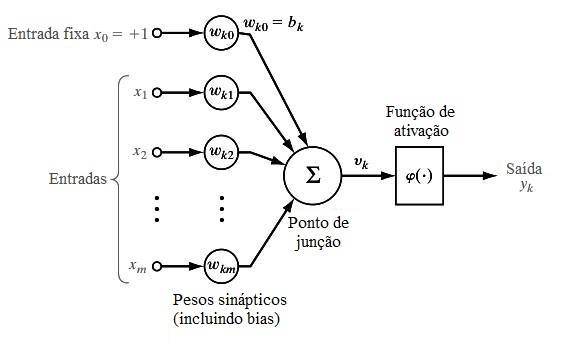
\includegraphics[width=0.8\textwidth]{./04-figuras/neuron-diagram-gray_traduzido}
    \fonte{Adaptado de \citeonline[p.~33]{Haykin1998}}
    \label{fig:neuronmodel}
\end{figure}

O modelo simples de um neurônio representado por perceptrons permite a simulação das já definidas sinapses, possibilitando a criação de RNAs complexas formadas por múltiplos neurônios, organizados em cadeias, como é mostrado na Figura \ref{fig:rna}. Neste exemplo, $x_1$, $x_2$ e $x_3$ são as entradas do sistema; os blocos 4, 5 e 6 representam, cada qual, um neurônio numa camada escondida; os blocos 7 e 8 representam os dois neurônios que compõem a camada de saída; e, por fim, $x_7$ e $x_8$ são as saídas de RNA. Redes como essa, que possuem mais de uma camada de neurônios, são denominadas \textit{Multilayer Perceptron} (MLP\footnote{Perceptron Multicamada (tradução nossa).}). As diferentes combinações que se podem obter distribuindo os neurônios de uma RNA de diferentes maneiras fazem com que estas redes possam ser utilizadas em aplicações diversas relacionadas à IA e IC.

\begin{figure}[!htb]
    \centering
    \caption{Modelo de um \textit{MLP}}
    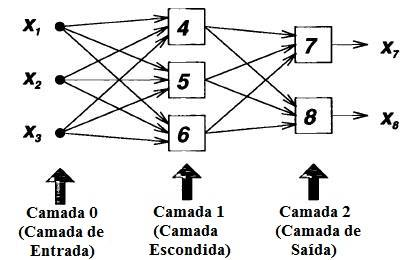
\includegraphics[width=0.6\textwidth]{./04-figuras/fund_teorica/rna_traduzido}
    \fonte{Adaptado de \citeonline[p.~205]{Jang1997}}
    \label{fig:rna}
\end{figure}

%vantagens das RNAs/ Funcionamento das RNAs
A principal característica de uma rede neural artificial que a torna interessante para aplicações computacionais é a sua capacidade de aprendizado. O procedimento usado para efetuar o processo de aprendizado é chamado \textit{algoritmo de aprendizado}, cuja função é modificar os pesos sinápticos da rede de forma ordenada para atingir um objetivo desejado \cite[p.~24]{Haykin1998}. É a partir deste aprendizado que as RNAs alcançam uma ótima taxa de generalização, fazendo delas fortes aliadas, por exemplo, para reconhecimento de padrões. Controladores que utilizam técnicas relacionadas a RNAs se beneficiam justamente destas capacidades de aprendizado e generalização conferidas por elas.

O controlador desenvolvido neste trabalho utiliza RNAs com treinamento supervisionado, que são treinadas a partir de um conjunto de entradas mapeadas no valor de suas respectivas saídas, resultando na obtenção de um conjunto de retas com parâmetros ajustados de acordo com os dados do treinamento. São as retas obtidas após este treinamento que conferem à rede o poder de generalização, permitindo que novas entradas sejam mapeadas para saídas que condizem com o cenário em questão.

Além disto, como o controlador projetado é do tipo Neuro-\textit{Fuzzy}, as retas ajustadas após o treinamento se enquadram num grupo especial correspondendo cada qual a uma função de pertinência de conjuntos \textit{Fuzzy}, assunto este que é abordado na seção seguinte.


\section{Lógica Fuzzy}
\label{sec:fundamentacaoTeorica-fuzzy}
%teoria de conjuntos fuzzy - pag 13 de jang
%inferencia fuzzy e raciocinio fuzzy - pag 47 jang

A lógica \textit{fuzzy} é uma alternativa à lógica convencional\footnote{lógica aristotélica.}, que permite uma abordagem diferente relacionada à pertinência de elementos a conjuntos implementando a possibilidade de se obter uma pertinência parcial para a definição desses conjuntos. A principal aplicação da lógica \textit{fuzzy} são os sistemas de inferência \textit{fuzzy}, tema que será abordado na Seção \ref{sec:sistema_inferencai_fuzzy}. As Seções \ref{sec:cojuntos_fuzzy}, \ref{sec:regras_fuzzy} e \ref{sec:raciocinio_fuzzy} referentes a conjuntos, regras e raciocínio \textit{fuzzy} respectivamente tratam dos diferentes componentes utilizados nestes sistemas. 
%e fazendo ainda uso de variáveis e termos linguísticos 

\subsection{Conjuntos \textit{Fuzzy}}
\label{sec:cojuntos_fuzzy}

Os conjunto \textit{fuzzy} são os componentes elementares dos sistema de inferência \textit{fuzzy} e se contrapõem àqueles definidos pela lógica tradicional, que restringe, aos valores 0 e 1, o grau de pertinência $\mu$ de um elemento $u$ a um conjunto $A$. Na lógica tradicional, este grau é definido da seguinte forma:
\begin{align*}
&\mu_A(u) = 1, \mbox{ se } u \mbox{ é um elemento do conjunto } A, \mbox{ e }\\
&\mu_A(u) = 0, \mbox{ se } u \mbox{ não é um elemento do conjunto } A
\end{align*}

Com isto, ou um elemento pertence a um conjunto ou não. Já os conjuntos \textit{fuzzy} permitem um grau de flexibilidade acerca do grau pertinência de cada elemento ao conjunto, sendo este grau definido por uma \textit{função de pertinência}. A definição formal de conjuntos \textit{fuzzy} e funções de pertinência é dada por \citeonline[p.~14]{Jang1997} como:
\begin{align*}
	A = \{(x,\mu_A(x)) \vert x \in X\}
\end{align*}

Nesta definição, um conjunto \textit{fuzzy} $A$ é composto pelos pares $(x,\mu_A(x))$ de cada elemento $x$ pertencente a um conjunto $X$, em que $x$ é o elemento em si e $\mu_A(x)$ é o grau de pertinência de $x$ ao conjunto $A$, que pode assumir qualquer valor entre 0 e 1, em que 0 representa a não-pertinência total do elemento ao conjunto e 1 representa a pertinência total a ele.

Como se pode perceber, a definição de um conjunto \textit{fuzzy} é uma simples extensão da referente a um conjunto clássico, no qual a função de pertinência (ou função característica) apenas pode assumir os valores 0 e 1. Se uma função de pertinência $\mu_A(x)$ de um conjunto \textit{fuzzy} $A$ é restrita a assumir os valores 0 ou 1, então ele é reduzido a um conjunto clássico \cite[p.~14]{Jang1997}.

Para melhor exemplificar a definição de conjuntos \textit{fuzzy}, tome como exemplo a Figura \ref{fig:fuzzy_sets_jang}. Neste caso, a variável idade (\textit{age}) é dividida em três subconjuntos \textit{fuzzy}, \textit{young, middle aged} e \textit{old}\footnote{jovem, meia idade e velho, respectivamente (tradução nossa).}, representados pelas funções de pertinência que os descrevem. Cada idade não precisa possuir necessariamente grau de pertinência 1 para algum conjunto e pode ainda pertencer simultaneamente a mais de um. A idade 30, por exemplo pertence ao conjunto jovem com grau de pertinência de 0,5 e também pertence ao conjunto meia idade com o mesmo grau.

\begin{figure}[!htb]
    \centering
    \caption{Funções de pertinência representando três conjuntos \textit{fuzzy} para a variável idade}
    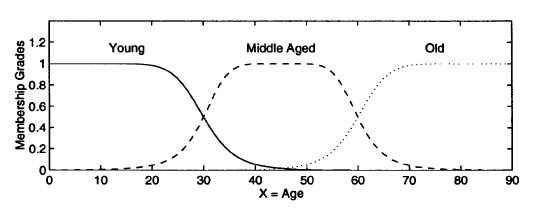
\includegraphics[width=0.8\textwidth]{./04-figuras/fund_teorica/fuzzy_sets_jang}
    \fonte{\citeonline[p.~17]{Jang1997}}
    \label{fig:fuzzy_sets_jang}
\end{figure}

Além dos conjuntos \textit{fuzzy}, há outro aspecto fundamental para o funcionamento desta lógica alternativa e poderosa: as regras \textit{fuzzy}.

%--revisao--
\subsection{Regras \textit{Fuzzy}}
\label{sec:regras_fuzzy}

As regras \textit{fuzzy} são os componentes de um sistema de inferência \textit{fuzzy} responsáveis por definir as relações entre as entradas do sistema e suas saídas e assumem a forma
\begin{center}
se $x$ é $A$ então $y$ é $B$
\end{center}
sendo ``$x$ é $A$'' denominada premissa  e ``$y$ é $B$'', consequente da regra em que $x$ e $y$ são \textit{variáveis linguísticas} de entrada e saída respectivamente  e $A$ e $B$ são os valores que elas assumem, representados por \textit{termos linguísticos}.

Uma variável linguística, segundo \citeonline[p.~54]{Jang1997}, é caracterizada por uma quíntupla $(x,T(x),X,G,M)$ em que $x$ é o nome da variável; $T(x)$ é o conjunto de termos de $x$, que é o conjunto de seus valores linguísticos ou termos linguísticos; $X$ é o universo de discurso; $G$ é uma regra sintática que gera os termos em $T(x)$; e $M$ é uma regra semântica que associa a cada termo linguístico A seu respectivo $M(A)$, em que $M(A)$ denota um conjunto \textit{fuzzy} em $X$.

Para facilitar a compreensão das definições relacionadas às variáveis linguísticas, o seguinte exemplo foi dado \cite[p.~55]{Jang1997}: se \textit{idade} é interpretado como uma variável linguística, então seu conjunto de termos $T(idade)$ poderia ser dado por:
\begin{align*}
\mbox{\textit{T(idade) = }}\{ &\mbox{ \textit{novo, não-novo, muito novo, não muito-novo,}} \dots, \\
&\mbox{ \textit{meia-idade, não de meia-idade,}} \dots, \\
&\mbox{ \textit{velho, não-velho, muito velho, mais ou menos velho, não muito velho,}} \dots, \\
&\mbox{ \textit{não muito novo e não muito velho,}} \dots \},
\end{align*}

Em que cada termo em $T(idade)$ é caracterizado por um conjunto \textit{fuzzy} de um universo de discurso $X = [0,100]$, como mostrado na Figura \ref{fig:fuzzy_rules_jang}. Geralmente, se diz ``idade é jovem'' para denotar a atribuição do valor linguístico jovem à variável linguística idade. A regra sintática se refere à forma como os valores linguísticos no conjunto de termos $T(idade)$ são gerados. A regra semântica define a função de pertinência de cada valor linguístico do conjunto de termos. A Figura \ref{fig:fuzzy_rules_jang} mostra algumas das funções de pertinência típicas para a variável linguística idade.

\begin{figure}[!htb]
    \centering
    \caption{Exemplo de função de pertinência do conjunto de termos T(idade)}
    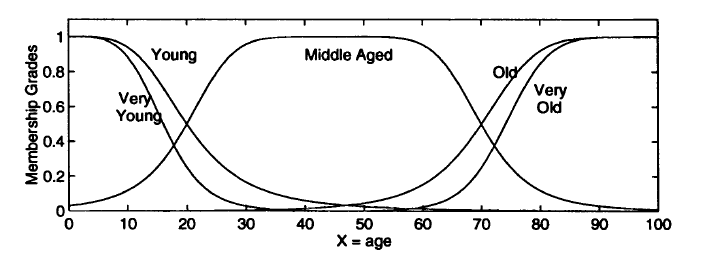
\includegraphics[width=0.8\textwidth]{./04-figuras/fund_teorica/fuzzy_rules_jang}
    \fonte{\citeonline[p.~55]{Jang1997}}
    \label{fig:fuzzy_rules_jang}
\end{figure}

Diversas regras \textit{fuzzy} fazem parte do nosso cotidiano. Exemplos possuindo a variável linguística \textit{idade} como variável linguística de entrada e saída respectivamente incluem:
\begin{center}
se \textit{idade} é \textit{jovem} então \textit{energia} é \textit{alta} \\
se \textit{sabedoria} é \textit{grande} então \textit{idade} é \textit{velha}
\end{center}

Um outro componente dos sistemas de inferência \textit{fuzzy} agrega muito valor ao uso de regras \textit{fuzzy}, permitindo a aplicação aproximada delas: o raciocínio \textit{fuzzy}.

\subsection{Raciocínio \textit{Fuzzy}}
\label{sec:raciocinio_fuzzy}

O processo de raciocínio \textit{fuzzy}, também conhecido como raciocínio aproximado, é um procedimento de inferência que deriva conclusões de um conjunto de regras \textit{fuzzy} \textit{se-então} como fatos conhecidos \cite[p.~62]{Jang1997} e é a partir dele que se pode fazer uma generalização a partir da regra básica na lógica tradicional com duas variáveis, denominada \textit{modus ponens}.

De acordo com a regra \textit{modus ponens}, podemos inferir a verdade da proposição $B$ a partir da verdade de $A$ e a implicação $A \rightarrow B$ (se A então B). Por exemplo, se $A$ é identifica por ``o tomate é vermelho'' e $B$ por ``o tomate está maduro'', então se é verdade que ``o tomate é vermelho'', é também verdade que ``o tomate está maduro''.

Contudo, o raciocínio humano emprega constantemente o modus ponens em uma maneira aproximada. Por exemplo, usando a mesma regra de implicação ``se o tomate é vermelho, então ele está maduro'', e sabemos que o ``o tomate está mais ou menos vermelho'' ($A^\prime$), então podemos inferir que ``o tomate está mais ou menos maduro'' ($B^\prime$), em que $A^\prime$ é próximo de $A$ e $B^\prime$ é próximo de $B$. Quando $A$, $B$, $A^\prime$ e $B^\prime$ são conjuntos \textit{fuzzy} do universo adequado, o procedimento de inferência descrito é chamado raciocínio aproximado ou raciocínio \textit{fuzzy}, podendo ser também chamado \textit{modus ponens} generalizado (GMP\footnote{Do inglês, \textit{Generalized Modus Ponens}}) \cite[p.~65]{Jang1997}.

A definição formal do raciocínio aproximado (raciocínio \textit{fuzzy}) é dada por \citeonline[p.~65]{Jang1997} como: sejam $A$, $A^\prime$, e $B$ conjuntos \textit{fuzzy} de $X$, $X$ e $Y$ respectivamente; assuma que a implicação \textit{fuzzy} $A \rightarrow B$ é expressa como uma relação $R$ em $X \times Y$. Então, o conjunto \textit{fuzzy} B induzido por ``$x$ é $A$'' e a regra \textit{fuzzy} ``se $x$ é $A$ então $y$ é $B$'' é definida por:
\begin{align*}
\mu_{B^\prime}(y) &= \max\nolimits_x \min[\mu_{A^\prime}, \mu_R(x,y)]
\\
&= \vee_x[\mu_{A^\prime}(x) \wedge \mu_R(x,y)], \\
\mbox{ou, equivalentemente,} \\
B^\prime &= A^\prime \circ R = A^\prime \circ (A \rightarrow B).
\end{align*}
 
Assim, podemos usar o procedimento de inferência do raciocínio \textit{fuzzy} para derivar conclusões, dado que a implicação \textit{fuzzy} $A \rightarrow B$ é definida como uma relação \textit{fuzzy} binária apropriada.

Uma vez definidos os conjuntos, regras e raciocínio \textit{fuzzy}, pode-se mostrar como eles são utilizados em conjunto pelos sistemas de inferência \textit{fuzzy}.
 
\subsection{Sistema de Inferência Fuzzy}
\label{sec:sistema_inferencai_fuzzy}

Um sistema de inferência fuzzy (FIS, do nome em inglês \textit{Fuzzy Inference System}) é uma ferramenta computacional popular e poderosa baseada nos conceitos de teoria de conjuntos fuzzy, regras fuzzy e raciocínio fuzzy. Há uma grande variedade de aplicações para sistemas de inferências fuzzy tais como controle automatizado, classificação de dados, análise de decisão, sistemas especialistas, predição de séries temporais, robótica e reconhecimento de padrões \cite[p.~73]{Jang1997}.

A estrutura básica de um FIS consiste de três componentes conceituais: uma base de regras, que contém uma seleção de regras fuzzy; um dicionário (ou base de dados), que define as funções de pertinência usadas nas regras fuzzy; e o mecanismo de raciocínio, que realiza o procedimento de inferência (geralmente o raciocínio fuzzy) sobre as regras e fatos dados para obter uma saída ou conclusão razoável \cite[p.~73]{Jang1997}. Sistemas de inferência fuzzy diferentes implementam estruturas ligeiramente diferentes entre si, havendo entretanto, três tipos principais de sistemas que podem ser aplicados aos mais diversos casos.

% corte 01
Os três principais tipos de FIS são os Mamdani, Tsukamoto e Sugeno e a diferença entre eles reside basicamente no consequente de suas regras fuzzy \cite[p.~74]{Jang1997}.

No sistema de inferência fuzzy Mamdani, o consequente das regras \textit{se-então} são conjuntos fuzzy. Desta forma, um sistema de inferências fuzzy Mamdani possui regras do seguinte tipo para um sistema com duas entradas e uma saída:
\begin{center}
se $x$ é $A$ e $y$ é $B$, então $z$ é $C$
\end{center}

Em que $x$, $y$ e $z$ são variáveis linguísticas nos universos de discurso $X$, $Y$ e $Z$, respectivamente e $A$, $B$ e $C$ são valores (termos) linguísticos. Com isto, um exemplo de sistema de inferências fuzzy Mamdani é formado pelas seguintes regras fuzzy:
\begin{align*}
\begin{cases}
&\mbox{Se }X  \mbox{é pequeno e } Y \mbox{é pequeno então } Z \mbox{ é muito negativo} \\
&\mbox{Se }X  \mbox{é pequeno e } Y \mbox{é grande então } Z \mbox{ é pouco negativo} \\
&\mbox{Se }X  \mbox{é grande e } Y \mbox{é pequeno então } Z \mbox{ é pouco positivo} \\
&\mbox{Se }X  \mbox{é grande e } Y \mbox{é grande então } Z \mbox{ é muito positivo} 
\end{cases}
\end{align*}

No caso do sistema de inferência fuzzy Tsukamoto, o consequente de cada regra fuzzy \textit{se-então} é representada por um conjunto fuzzy com uma função de pertinência monotônica\footnote{Uma função sempre crescente ou sempre decresente; uma função cuja derivada nunca muda de sinal}. Um exemplo de modelo fuzzy Tsukamoto de entrada única pode ser expressa como:
\begin{align*}
\begin{cases}
&\mbox{Se }X  \mbox{é pequeno então } Y \mbox{ é } C_1\\
&\mbox{Se }X  \mbox{é médio então } Y \mbox{ é } C_2\\
&\mbox{Se }X  \mbox{é grande então } Y \mbox{ é } C_3
\end{cases}
\end{align*}

No sistema de inferência fuzzy Sugeno, também conhecido como TSK (Takagi-Sugeno-Kang), o consequente é um função envolvendo as variáveis de entrada. Com isto, uma regra fuzzy típica de um modelo fuzzy Sugeno possui a seguinte forma:
\begin{center}
se $x$ é $A$ e $y$ é $B$, então $z = f(x,y)$,
\end{center}

Em que $A$ e $B$ são conjuntos fuzzy do antecedente, enquanto $z = f(x,y)$ é uma função no consequente. Geralmente, $f(x,y)$ é uma função polinomial sobre as variáveis $x$ e $y$, mas pode ser qualquer função, contanto que seja capaz de descrever apropriadamente a saída do modelo dentro da região fuzzy especificada pelo antecedente da regra. Um exemplo de sistema de inferências fuzzy TSK com duas entradas e uma saída é formado pelas seguintes regras fuzzy:
\begin{align*}
\begin{cases}
&\mbox{Se }X  \mbox{é pequeno e } Y \mbox{é pequeno então } z=-x+y+1 \\
&\mbox{Se }X  \mbox{é pequeno e } Y \mbox{é grande então } z=-y+3  \\
&\mbox{Se }X  \mbox{é grande e } Y \mbox{é pequeno então } z=-x+3  \\
&\mbox{Se }X  \mbox{é grande e } Y \mbox{é grande então } z=x+y+2  
\end{cases}
\end{align*}

Esta propriedade dos sistemas de inferência fuzzy Sugeno de possuírem, como consequente, funções paramétricas que relacionam as premissas abre várias possibilidades para sua aplicação. Uma delas é implementada por uma técnica que alia o poder das RNAs ao do FIS: o sistema de inferência neuro-fuzzy.

%Esta propriedade dos sistemas de inferência fuzzy Sugeno de possuírem, como consequente, uma função que relaciona as premissas abre várias possibilidades para sua aplicação. Uma delas é implementada por uma técnica que alia o poder de aprendizado e generalização das RNAs ao uso de variáveis linguísticas, definições de pertinência parciais e raciocínios aproximados da lógica fuzzy: o sistema de inferência neuro-fuzzy.

% corte 01
%Um sistema de inferência fuzzy pode tomar entradas fuzzy ou \textit{crisp}, mas as saídas que ele produz são sempre conjuntos fuzzy. Algumas vezes, é necessário se obter uma saída \textit{crisp}, principalmente quando o sistema de inferência fuzzy é usado como um controlador. Desta forma, se faz necessário um método de defuzzificação para extrair um valor \textit{crisp} que melhor represente um conjunto fuzzy.

%Com entradas e saídas \textit{crisp}, um sistema de inferência fuzzy implementa um mapeamento não linear do espaço de entrada para o espaço de saída. Este mapeamento é realizado por um número de regras fuzzy \textit{se-então}, cada qual descrevendo o comportamento local do mapeamento. Em particular, o antecedente de uma regra define a região fuzzy no espaço de entrada, enquanto o consequente especifica a saída na região fuzzy \cite[p.~73]{Jang1997}.

%\section{\textit{Soft Computing} e Neuro-Fuzzy}
\section{Redes Neuro-\textit{Fuzzy}}
\label{sec:fundamentacaoTeorica-neuro-fuzzy}
%Página 1 (introdução); Página 333 (Neuro-Fuzzy Modeling) de Jang1997
%
%De Jang1997, incluir mais texto
%	Fuzzy: Mamdani, Sugeno, TSK
%	RNA: Aprendizado supervisionado x não-supervisionado; aprendizado por reinforcement

Aliando o poder das RNAs, que reconhecem padrões e se adaptam para lidar com mudanças no ambiente, aos sistemas de inferência \textit{fuzzy}, que incorporam o conhecimento humano e executam inferências e tomadas de decisão, surgiram os sistemas de inferência neuro-\textit{fuzzy} (ANFIS, acrônimo para \textit{Adaptive Neuro-Fuzzy Inference System}), uma nova ferramenta computacional poderosa amplamente utilizada em diversos contextos \cite[p.~1]{Jang1997}.

\subsection{ANFIS: \textit{Adaptive Neuro-Fuzzy Inference Systems}}
Segundo \citeonline[p.~335]{Jang1997}, do ponto de vista funcional, praticamente não há limitações para a gama de funções, no sentido matemático, de uma rede neuro-\textit{fuzzy}, exceto pela exigência de ela ser diferenciável por partes. Devido às mínimas restrições, redes neuro-\textit{fuzzy} podem ser empregadas diretamente em uma grande variedade de aplicações de modelagem, tomadas de decisão, processamento de sinal e controle.

%\subsubsection{Arquitetura ANFIS}
Para simplificar, a arquitetura ANFIS\footnote{Sistema de Inferência Neuro-\textit{Fuzzy} Adaptativo (tradução nossa).} será descrita considerando-a dotada de duas entradas $x$ e $y$ e uma saída $z$. Para um modelo \textit{fuzzy} Sugeno de primeira ordem, um conjunto comum de regras do tipo \textit{se-então} é o seguinte:

\begin{center}
    Regra 1: Se $x$ é $A_1$ e $y$ é $B_1$, então $f_1 = p_1x + q_1y + r_1$,\\
    Regra 2: Se $x$ é $A_2$ e $y$ é $B_2$, então $f_2 = p_2x + q_2y + r_2$. 
\end{center}

A Figura \ref{fig:anfis} ilustra um mecanismo de raciocínio para o modelo Sugeno e a arquitetura ANFIS equivalente, em que nós de uma mesma camada têm funções similares, como descrito a seguir.
\begin{figure}[!htb]
    \centering
    \caption{Equivalência entre modelo \textit{fuzzy} Sugeno e ANFIS; (a) Um modelo \textit{fuzzy} Sugeno com duas entradas de primeira ordem com duas regras; (b) arquitetura ANIFS equivalente}
    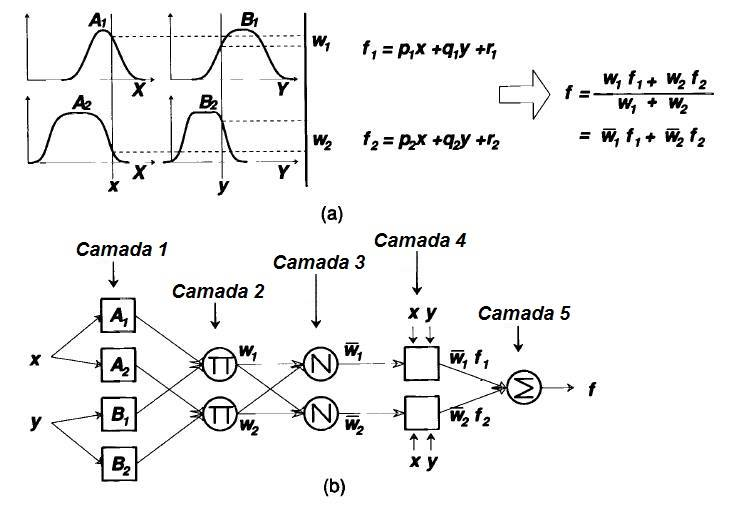
\includegraphics[width=0.8\textwidth]{./04-figuras/fund_teorica/anfis_traduzido}
    \fonte{\cite[p.~336]{Jang1997}}
    \label{fig:anfis}
\end{figure}

Na camada 1 (\textit{Layer 1}), todo nó \textit{i} é um nó adaptativo com uma função de nó do tipo:
\begin{align*}
    O_{1,i} = \mu_{A_{i}}(x), \mbox{ para } i = 1, 2, \mbox{ ou}\\
    O_{1,i} = \mu_{B_{i-2}}(y), \mbox{ para } i = 3, 4
\end{align*}
em que $x$ (ou $y$) é a entrada para o nó $i$ e $A_{i}$ (ou $B_{i-2}$) é um termo linguístico (como ``pequeno'' ou ``grande'') associado a este nó. Em outras palavras, $O_{1,i}$ é o grau de pertinência de um conjunto \textit{fuzzy} $A$ ($A_1$, $A_2$, $B_1$ ou $B_2$) e especifica o grau em que a entrada $x$ (ou $y$) satisfaz o quantificador $A$. Aqui, a função de pertinência $A$ pode ser qualquer função de pertinência parametrizada apropriada. Parâmetros nesta camada são chamados parâmetros de premissa \cite[p.~336]{Jang1997}.

Na camada 2 (\textit{Layer 2}), cada nó é um nó fixo rotulado $\prod$, cuja saída é o produto de todos sinais de entrada:
\begin{align*}
    O_{2,i} = w_i = \mu_{A_{i}}(x)\mu_{B_{i-2}}(y), i = 1, 2.
\end{align*}

Cada nó de saída representa a força de ativação de uma regra. Em geral, qualquer outro operador norma-T\footnote{Operador de interseção \cite[p.~337]{Jang1997}} que desempenhe a operação \textit{AND} \textit{fuzzy} pode ser usado como função de nó nesta camada \cite[p.~337]{Jang1997}.

Na camada 3 (\textit{Layer 3}), cada nó é um nó fixo rotulado N. O $i$-ésimo nó calcula a taxa da força de ativação da $i$-ésima regra pela soma da força de ativação de todas as regras:
\begin{align*}
    O_{3,i} = \bar{w_i} = \frac{w_i}{w_1 + w_2}, i = 1, 2.
\end{align*}

Por conveniência, saídas desta camada são chamadas forças de ativação normalizadas \cite[p.~336]{Jang1997}.

Na camada 4 (\textit{Layer 4}), todo nó $i$ é um nó adaptativo com uma função nodal
\begin{align*}
    O_{4,i} = \bar{w_i}f_i = \bar{w_i}(p_ix+q_iy+r_i),
\end{align*}
em que $\bar{w_i}$ é um taxa da força de ativação normalizada da camada 3 e \{$p_i, q_i, r_i$\} é o conjunto de parâmetros deste nó. Parâmetros nesta camada são denominados parâmetros consequentes \cite[p.~336]{Jang1997}.

O único nó na camada 5 (\textit{Layer 5}) é um nó fixo denominado $\sum$, e é responsável por computar a saída global como a soma ponderada de todos os sinais de entrada:
\begin{align*}
    \mbox{saída global} = O_{5,i} = \sum_{i} {\bar{w_i}f_i} = \frac{\sum_{i} {w_if_i}}{\sum_{i} {w_i}} %\overline{w_i}(p_ix+q_iy+r_i),
\end{align*}

Com esta arquitetura, constrói-se uma rede neuro-\textit{fuzzy} (ANFIS) que é funcionalmente equivalente a um modelo \textit{fuzzy} Sugeno \cite{Jang1997}. Com isto, sistemas de inferência neuro-\textit{fuzzy} podem operar, por exemplo, utilizando o treinamento supervisionado de uma RNA para ajustar o valor dos parâmetros das funções de resposta dos sistemas de inferência \textit{fuzzy} Sugeno para uma dada operação. Um exemplo de aplicação para este tipo de rede seria o controle de sistemas não lineares.

\subsection{Controladores \textit{Fuzzy} e Neuro-\textit{Fuzzy}}
%Página 451 (Neuro-Fuzzy Control) de Jang1997

Um controlador lógico fuzzy (FLC)\footnote{Do inglês, \textit{Fuzzy Logic Controller}.} é um sistema de inferência fuzzy projetado especificamente para atuar como controlador de um sistema que se deseja controlar. Este FIS portanto possui, como entradas, sinais provenientes do sistema e, como saídas, sinais de atuação sobre ele.

Com o avanço dos microprocessadores e hardware, tem se criado uma diversidade ainda maior de domínios para aplicação de controladores lógicos fuzzy, que vão de eletroeletrônicos à indústria automobilística. De fato, para sistemas complexos ou mal definidos que não são facilmente sujeitados a métodos de controle convencionais, os FLCs proveem uma alternativa viável, uma vez que eles podem capturar os aspectos qualitativos aproximados do raciocínio de um humano e o processo de tomada de decisão. De qualquer forma, sem a capacidade adaptativa, a performance de um FLC se baseia exclusivamente em dois fatores: a disponibilidade de humanos com expertise e as técnicas de aquisição de conhecimento para converter esta expertise humana nas apropriadas regras fuzzy \textit{se-então} e funções de pertinência. Estes dois fatores restringem substancialmente o domínio de aplicações dos FLCs \cite[p.~451]{Jang1997}.

Nesse contexto, o uso de controladores neuro-fuzzy passou a se mostrar muito interessante, tendo em vista que eles eliminam os dois fatores citados que restringem bastante o domínio de aplicações dos FLCs, uma vez que os sistemas ANFIS preenchem as lacunas deixadas pelos FIS, eliminando a necessidade de humanos com expertise sobre o sistema e encorporando técnicas de aquisição de conhecimento.

Com isto, podem-se identificar algumas propriedades particulares aos controladores ANFIS que os tornam ótimas opções para diversos casos \cite[p.~458]{Jang1997}:
\begin{enumerate}
  \item Habilidade de aprendizado;
  \item Operação paralela;
  \item Representação do conhecimento estruturado;
  \item Melhor integração com outros métodos de controle.
\end{enumerate}

Como comparativo, é importante salientar que uma RNA possui as propriedades 1 e 2, mas não as 3 e 4, que são devidas à contribuição dos sistemas de inferência fuzzy \cite[p.~458]{Jang1997}. Um ANFIS, por aliar as duas técnicas, possui todas essas propriedades.

Ainda segundo o autor, há diversas formas diferentes de se projetar controladores neuro-fuzzy. A maioria deles são não lineares. Assim sendo, uma análise rigorosa para sistemas de controle neuro-fuzzy é difícil e continua sendo uma área desafiadora para outras investigações. Por outro lado, um controlador neuro-fuzzy geralmente contém um grande número de parâmetros, o que o torna mais versátil do que um controlador linear ao lidar com características não lineares de plantas. Desta forma, controladores neuro-fuzzy quase sempre superam controladores puramente lineares se devidamente projetados.

%Por outro lado, investigações usando redes neurais em sistemas de controle automatizados não receberam muita atenção até que a regra de aprendizado com \textit{backpropagaion} fosse reformulada em 1986. Desde então, pesquisas de controle neural têm evoluído rapidamente e um grande número de métodos que o implementam tem sido proposto na literatura \cite[p.~451]{Jang1997}.

%\subsubsection{Sistemas de Controle Realimentados}
%A \autoref{fig:feedback-control-system-diagram} é um diagrama de blocos de um típico sistema de controle realimentado, em que a planta (ou processo) representa o sistema dinâmico a ser controlado e o controlador emprega uma estratégia de controle para alcançar um objetivo proposto.
%
%\begin{figure}[!htb]
%    \centering
%    \caption{Diagrama de blocos de um sistema de controle realimentado}
%    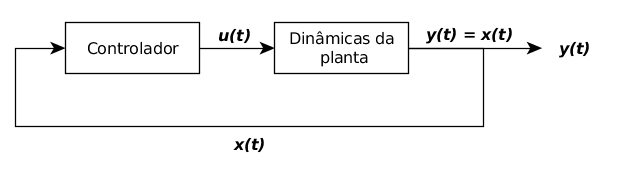
\includegraphics[width=0.9\textwidth]{./04-figuras/Jang1997_feedback_control_system_diagram}
%    \fonte{Adaptado de \citeonline[p.~455]{Jang1997}}
%    \label{fig:feedback-control-system-diagram}
%\end{figure}

%\subsubsection{Controlador Neuro-Fuzzy}
%Se o controlador da \autoref{fig:feedback-control-system-diagram} for substituído por RNAs ou sistemas de inferência fuzzy, obteríamos sistemas de controle neural ou fuzzy, respectivamente. Em outras palavras, métodos de controle neurais ou fuzzy são formas sistemáticas de construir redes neurais ou sistemas de inferência fuzzy como controladores com a intenção de se alcançar um objetivo de controle pré-estabelecido. Da mesma forma, um controle neuro-fuzzy se refere à concepção de métodos para controladores de lógica fuzzy que empregam técnicas de redes neurais. Em particular, podem-se citar métodos para ANFIS \cite[p.~458]{Jang1997}.





%\citeonline[p.~1]{Jang1997} define \textit{Soft Computing}\footnote{Computação Flexível, tradução nossa} (SC) como uma abordagem inovadora para construir sistemas inteligentes computacionais. Segundo ele, chegou-se a um momento em que soluções eficientes para problemas do mundo real requerem sistemas inteligentes que combinem conhecimento, técnicas e metodologias de diferentes fontes. Estes sistemas inteligentes deveriam possuir expertise humanóide com um domínio específico, se adaptar e aprender a agir melhor em mundanças de ambientes e explicar como eles tomam as decisões ou tomam ações.
%
%
%Os diferentes paradigmas que constituem a \textit{Soft Computing} incluem redes neurais, teoria de conjuntos fuzzy, métodos de otimização tais como algoritmos genéticos e \textit{simulated annealing}. Cada um destes métodos possui seu próprio ponto forte, como é mostrado no \autoref{qua:Jang1997_sc_constituents}. A integração adequada destas metodologias formam o núcleo da SC; a sinergia permite à SC a incorporar o conhecimento humano efetivamente, lidar com imprecisão e incerteza, e aprender para se adaptar a diferentes ou desconhecidos ambientes para melhor performance \cite[p.~2]{Jang1997}.
%
%\begin{quadro}[!htb]
    \centering
    \caption{Constituintes da \textit{Soft Computing} e inteligência artificial convencional\label{qua:Jang1997_sc_constituents}}
    \begin{tabular}{|c|c|}
        \hline
            \textbf{Medologia} & 
            \textbf{Ponto Forte} \\
        \hline
            Rede Neural &
            Aprendizado e Adaptção \\
        \hline
            \multirow{2}{*}{Teoria de Conjuntos Fuzzy}&Representação do conhecimento\\
            &via regras se-então\\
        \hline
            Algoritmos Genéticos e \textit{simulated annealing} &
            Pesquisa randômica sistemática \\

        % \hline
        %     \shortstack{Algoritmos Genéticos e \\ \textit{simulated annealing}} &
        %     Pesquisa randômica sistemática\\

        % \hline
        %     \multirow{2}{*}{\shortstack{Algoritmos Genéticos e \\ \textit{simulated annealing}}} &
        %     Pesquisa randômica sistemática\\

        \hline
            IA Convencional &
            Manipulação Simbólica \\
        \hline
    \end{tabular}
    \fonte{Adaptado de \citeonline[p.~2]{Jang1997}}
\end{quadro}


